\section{Tracking Performance}\label{sec:trackingPerformance}

The momentum resolution $\sigma(\Delta p/{p^{2}}_{True})$ as well as the
transverse $\sigma(\Delta d_{0})$ and longitudinal $\sigma(\Delta z_{0})$ impact parameter resolutions are compared for the different implemented geometries using single muons with momenta of 1, 10 and 100~GeV for different polar and azimuthal angles. The resolutions are obtained from a Gaussian fit using at least 10000 simulated events and reconstructed tracks.
The statistical errors on the impact parameter resolutions are also given in the plots and they are negligible.

\subsection{The \emph{spirals} geometry}

%% The momentum and the transverse and longitudinal impact parameter resolutions are computed for the CDR and the spirals geometries using single muons with a polar angle of $\theta = 20^\circ$ and momenta of 1, 10 and 100~GeV as shown in Figure \ref{fig:spiralRes}. The points are obtained from a Gaussian fit using at least 10000 simulated events and reconstructed tracks. \\
To study the impact of the \begin{it}spirals\end{it} geometry on the tracking performance, single muons are used with a polar angle of $\theta=20^{\circ}$ and azimuthal angles of $\phi=180^{\circ}$ or $\phi=225^{\circ}$ which hit the first and the last modules of the first endcap layer, respectively. Figure~\ref{fig:spiralRes} compares the $p$, $d_{0}$ and $z_{0}$ resolutions for the CDR and the \begin{it}spirals\end{it} geometries. \\
%% In Figure \ref{fig:spiralRes} we also want to see how much the resolution changes from one module of the endcap to the other as the modules for each endcap layer are situated in different z positions. For this purpose, we have chosen two different azimuthal angles $\phi=180^\circ$ and $\phi=135^\circ$ which respectively correspond to the first module and the last module of the first endcap layer as shown in Figure \ref{fig:spiralEndcapsPhis}.
The momentum resolutions are very similar in all cases as the measurement of the momentum is dominated by the main tracker. The spiral arrangement affects the $d_0$ and $z_0$ resolutions in the forward direction. This can be explained by the fact that the measurement of these two parameters depends on the distance of the vertex layers to the interaction point. \\
These results are in a reasonable agreement with the results presented in the CDR.

\begin{figure}[H]
  %\hspace{-2cm}
        %\centering
        \begin{subfigure}[b]{0.4\textwidth}
          \centering
          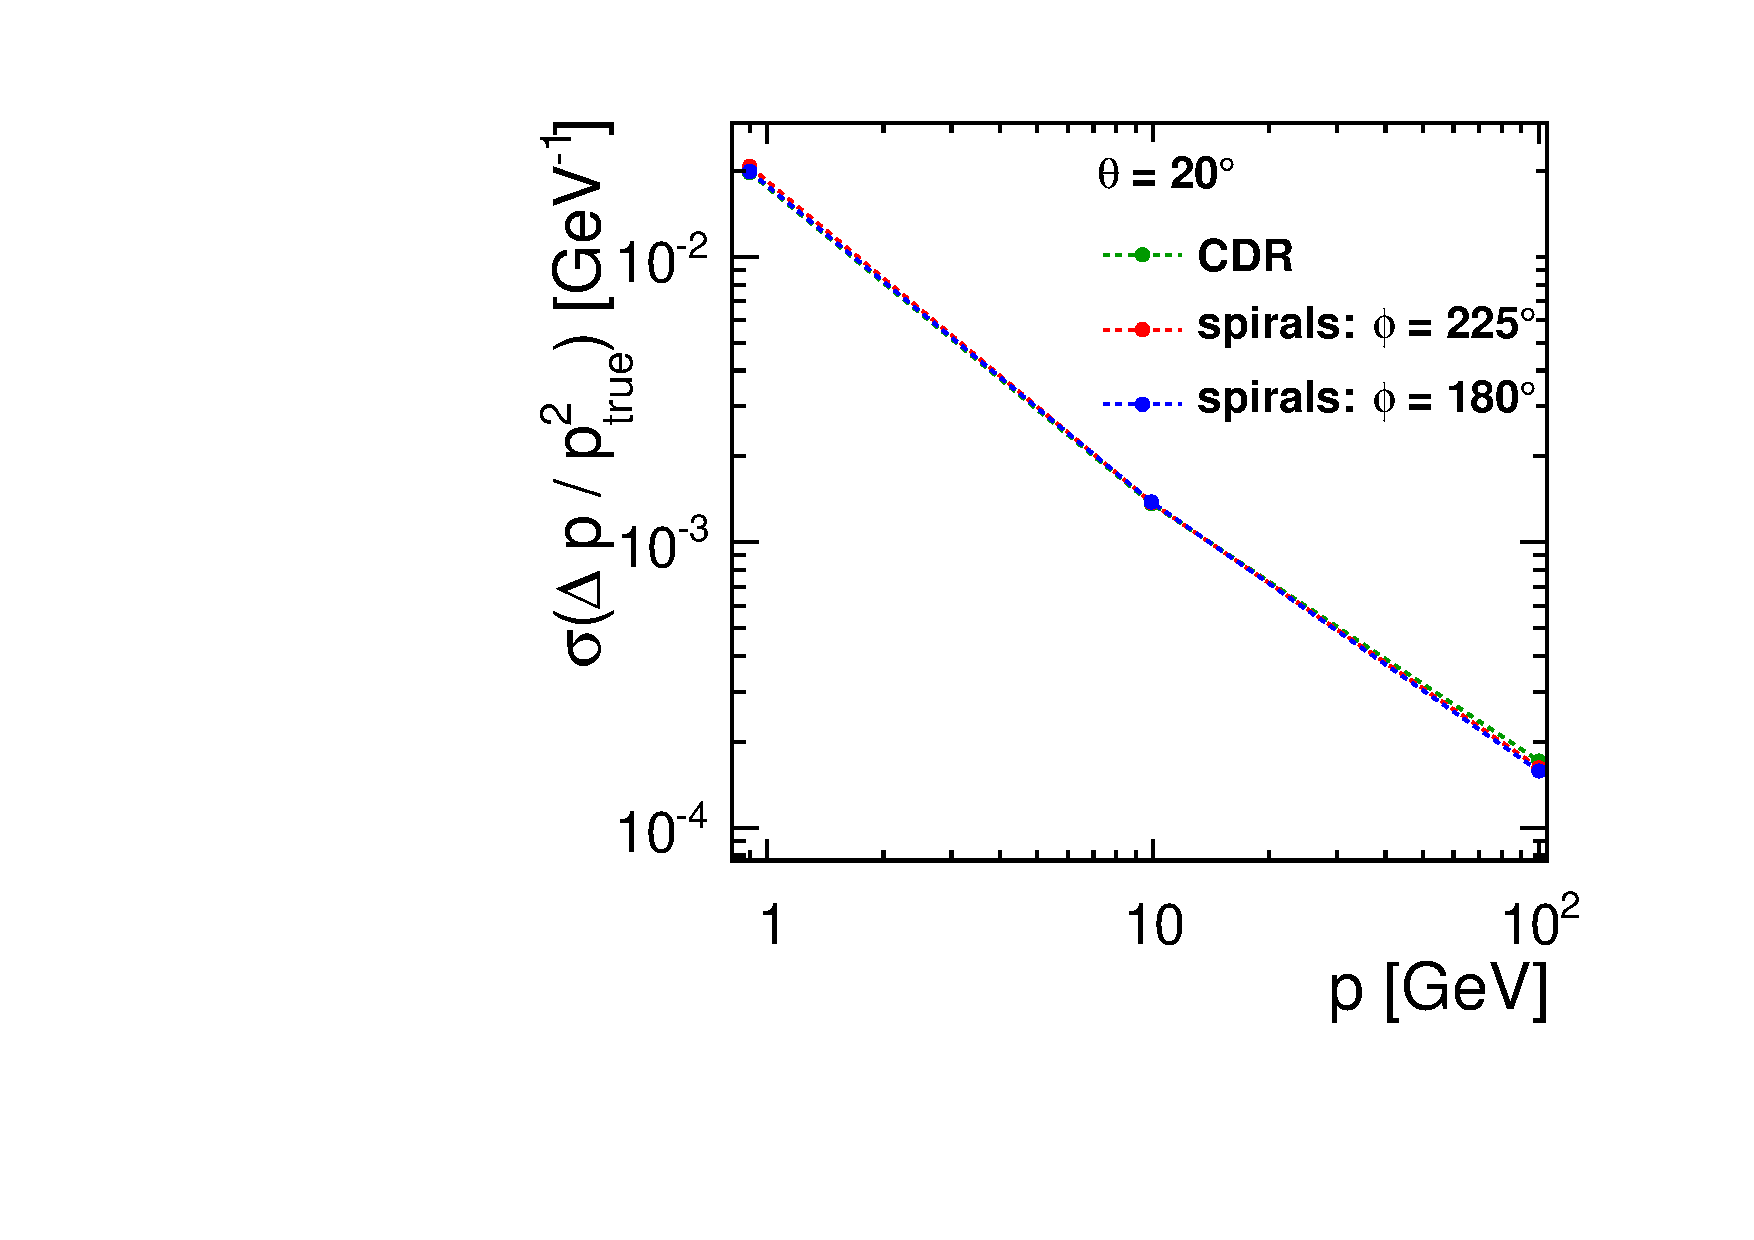
\includegraphics[width=\textwidth]{Figures/Geometries/pT_resolution_spirals.pdf}
          \caption{Momentum resolution}
          \label{}
        \end{subfigure}%
        ~ 
        \begin{subfigure}[b]{0.4\textwidth}
          \centering
          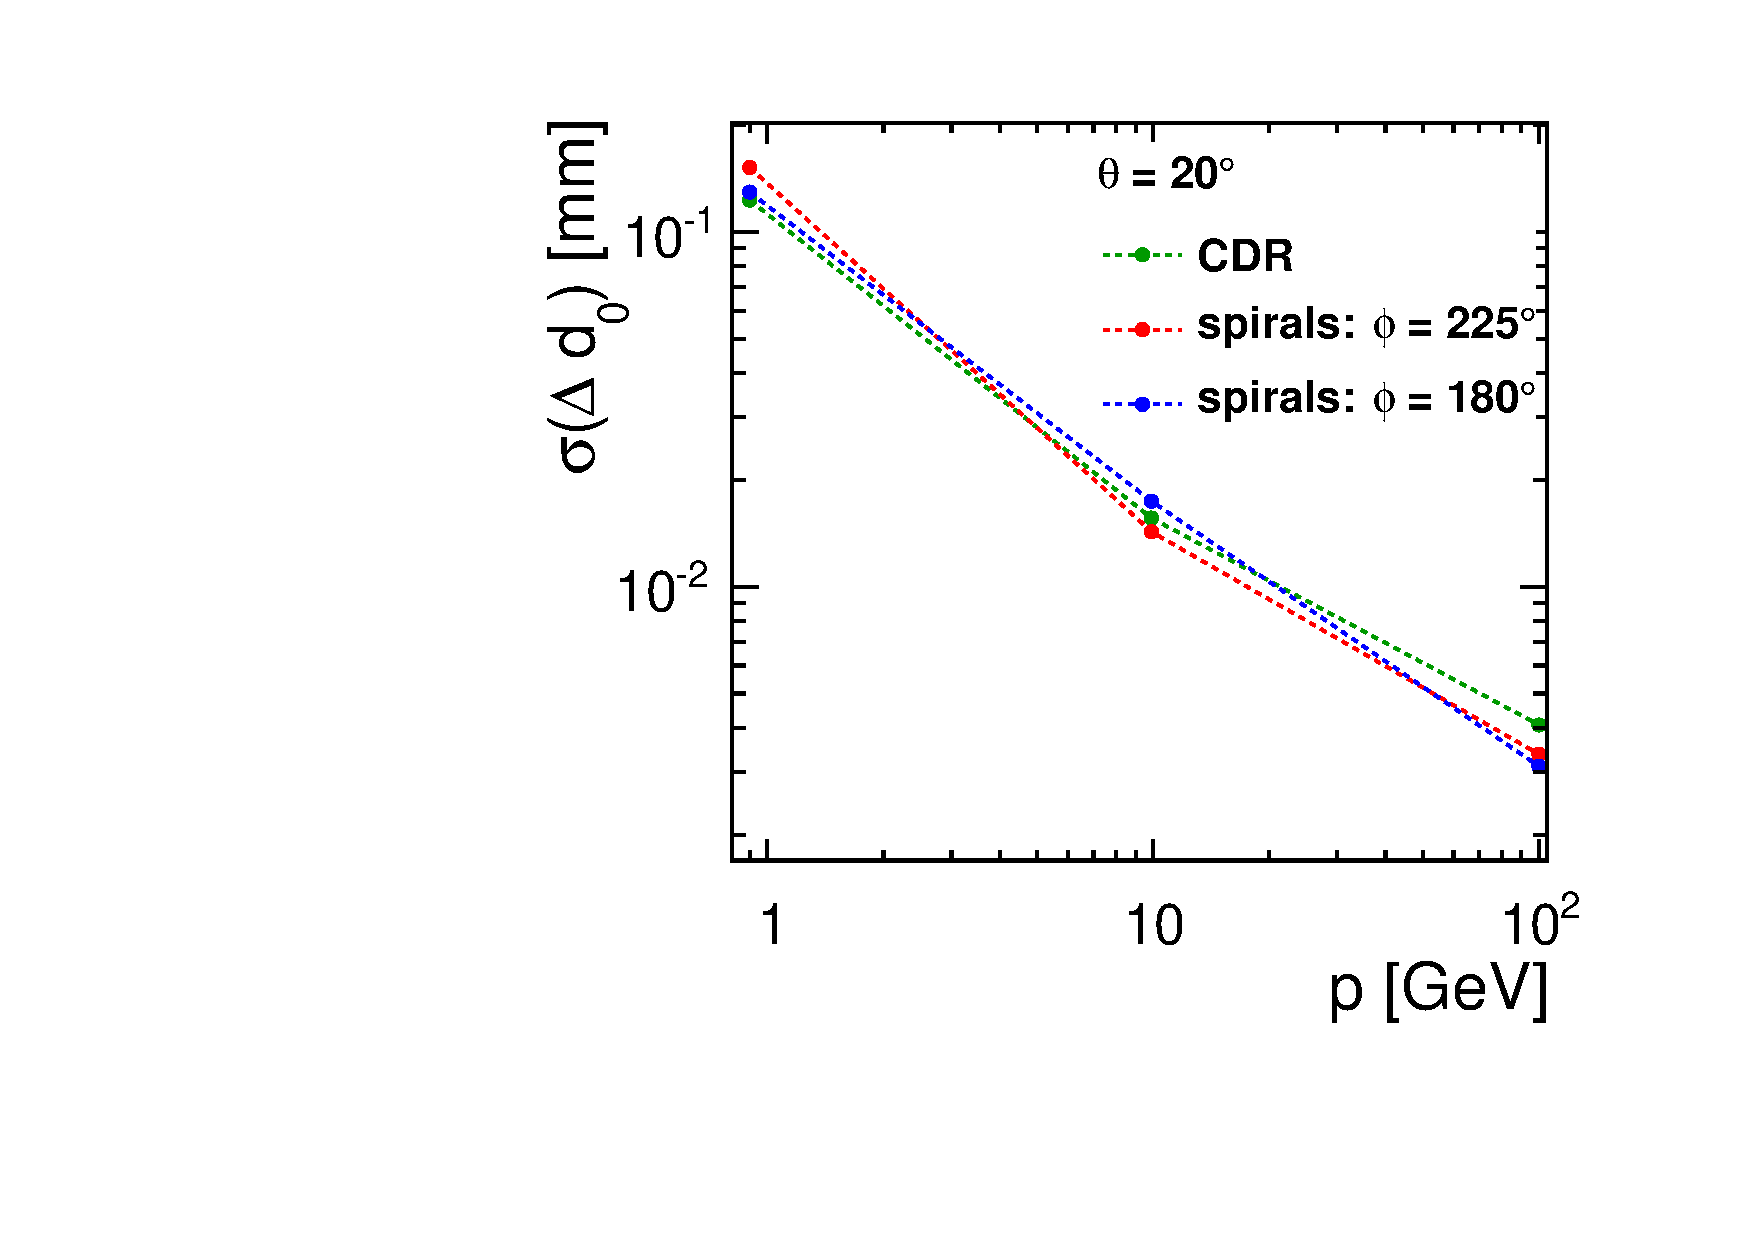
\includegraphics[width=\textwidth]{Figures/Geometries/d0_resolution_spirals.pdf}
          \caption{Transverse impact-parameter resolution}
          \label{}
        \end{subfigure}
        ~
        \begin{subfigure}[b]{\textwidth}
          \centering
          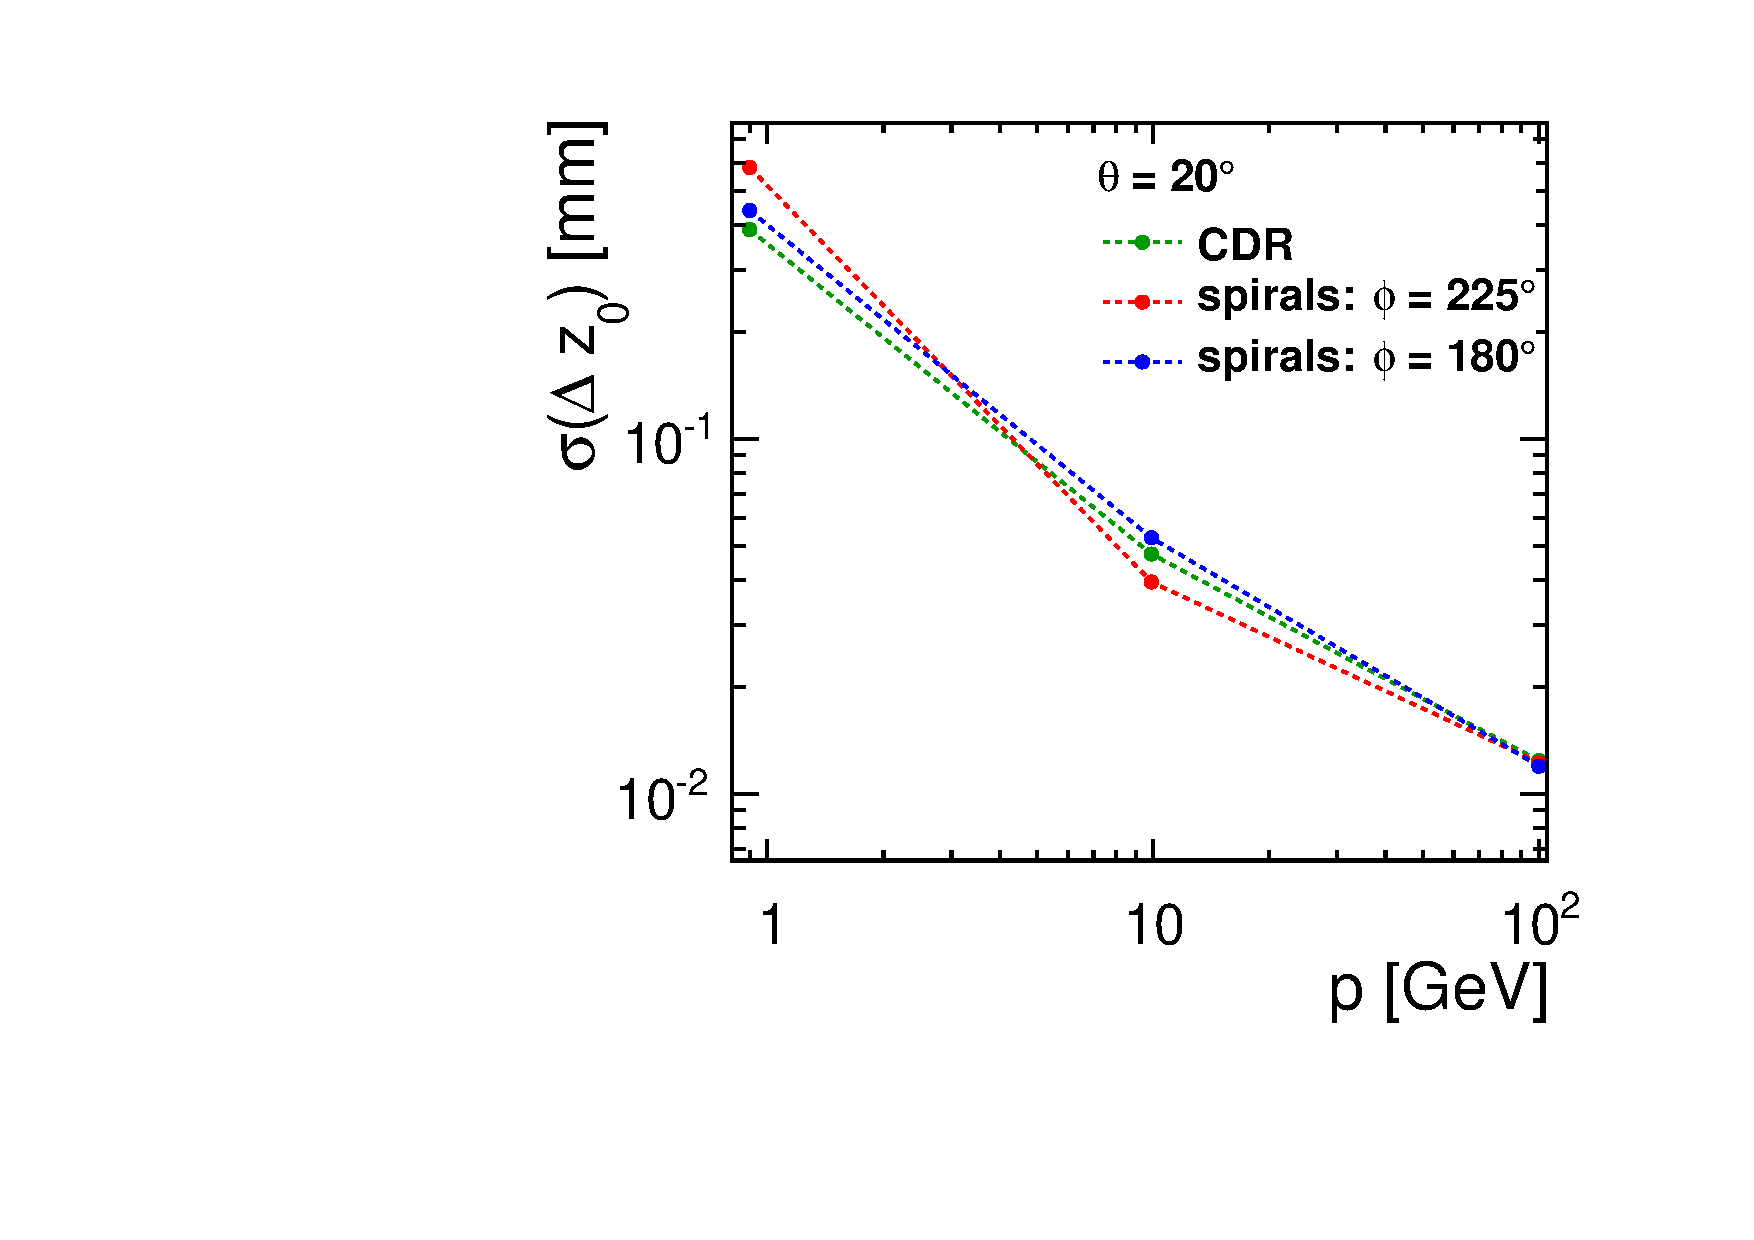
\includegraphics[width=0.4\textwidth]{Figures/Geometries/z0_resolution_spirals.pdf}
          \caption{Longitudinal impact-parameter resolution}
          \label{}
        \end{subfigure}
        \caption{(a) Momentum, (b) transverse impact-parameter and
          (c) longitudinal impact-parameter resolutions for the CDR and
          the {\it spirals} geometries for single muons at $\theta = 20^\circ$.}\label{fig:spiralRes}
\end{figure}


\subsection{The \emph{double\_spirals} geometry}
The effect of the \begin{it}double\_spirals\end{it} geometry on the tracking performance in the barrel region is studied for single muons with a polar angle of $\theta=90^\circ$ in Figure~\ref{fig:doubleLayerRes}.


\begin{figure}[H]
        \centering
        \begin{subfigure}[b]{0.4\textwidth}
          \centering
          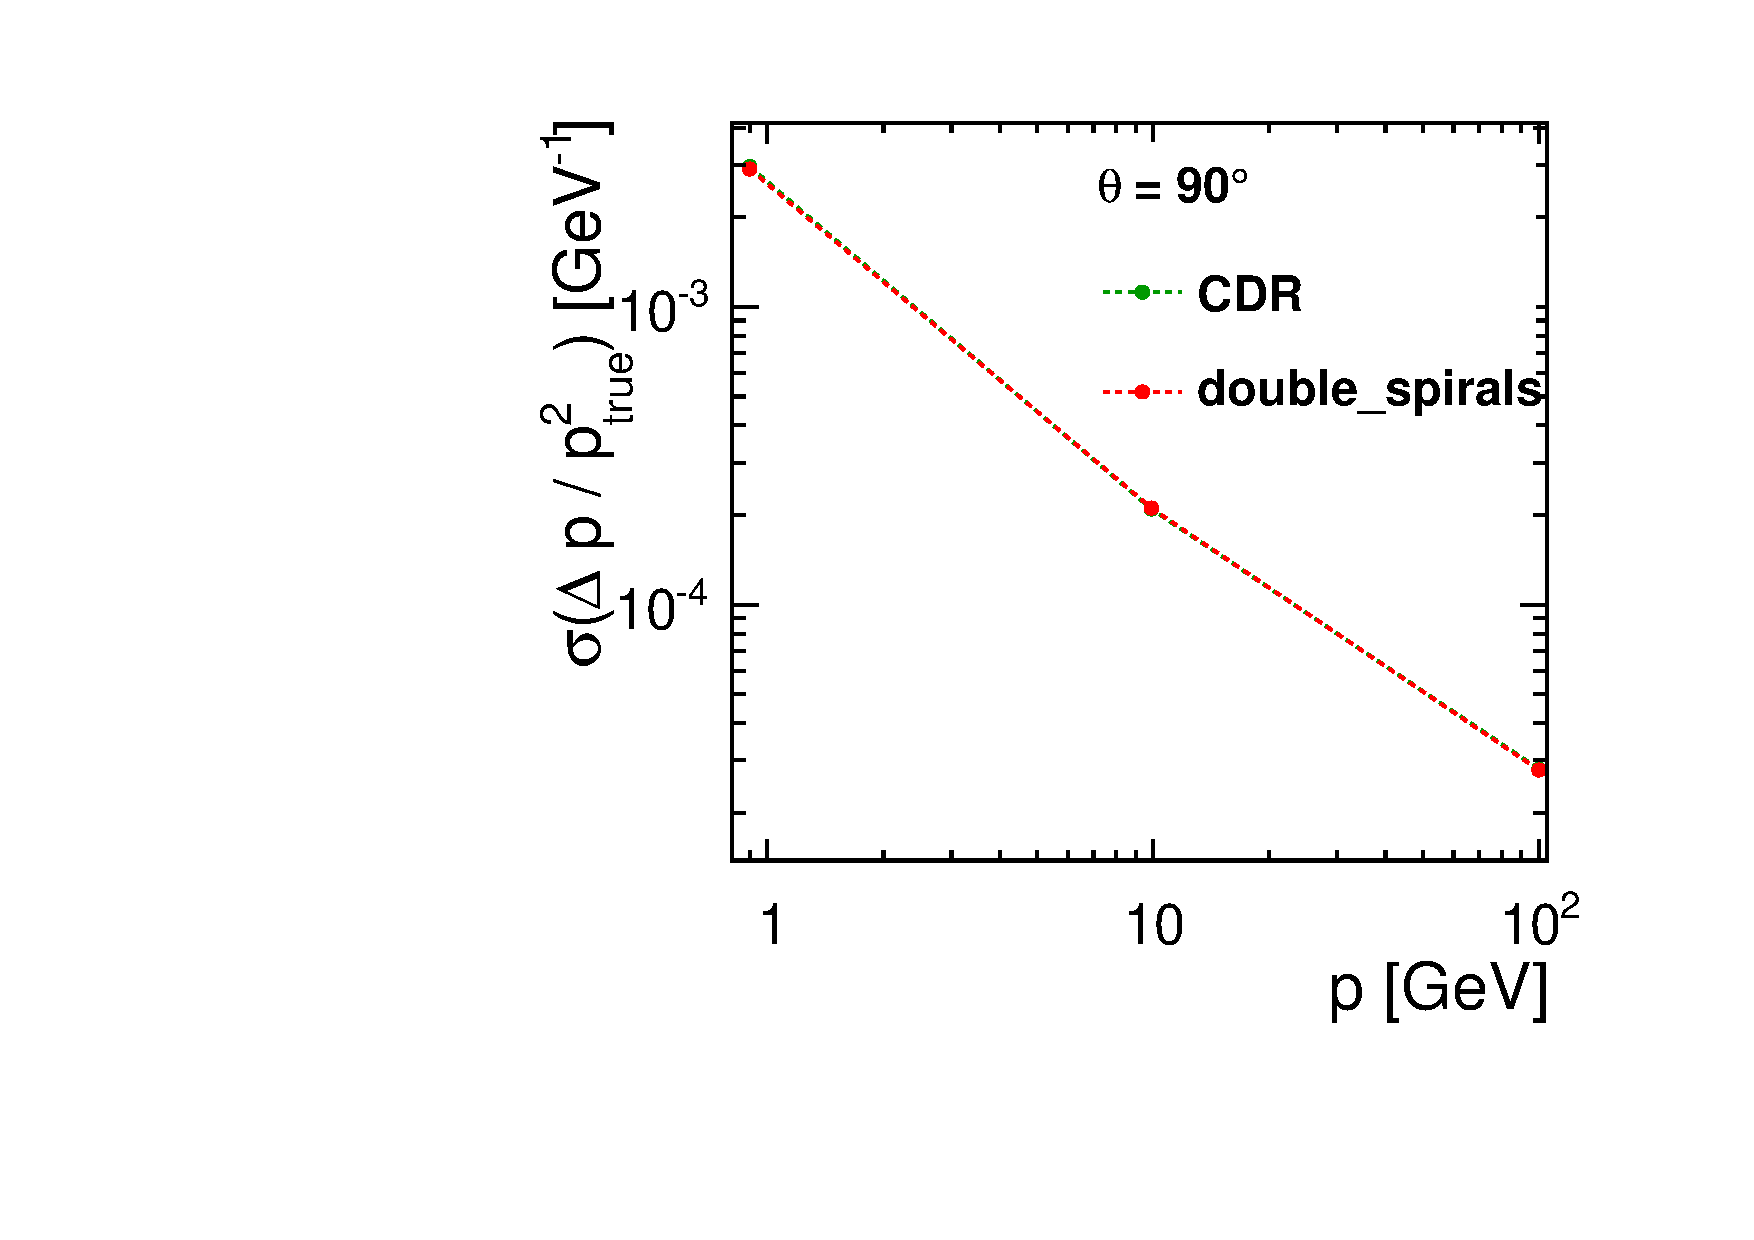
\includegraphics[width=\textwidth]{Figures/Geometries/pT_resolution_double.pdf}
          \caption{Momentum resolution}
          \label{}
        \end{subfigure}%
        ~ 
        \begin{subfigure}[b]{0.4\textwidth}
          \centering
          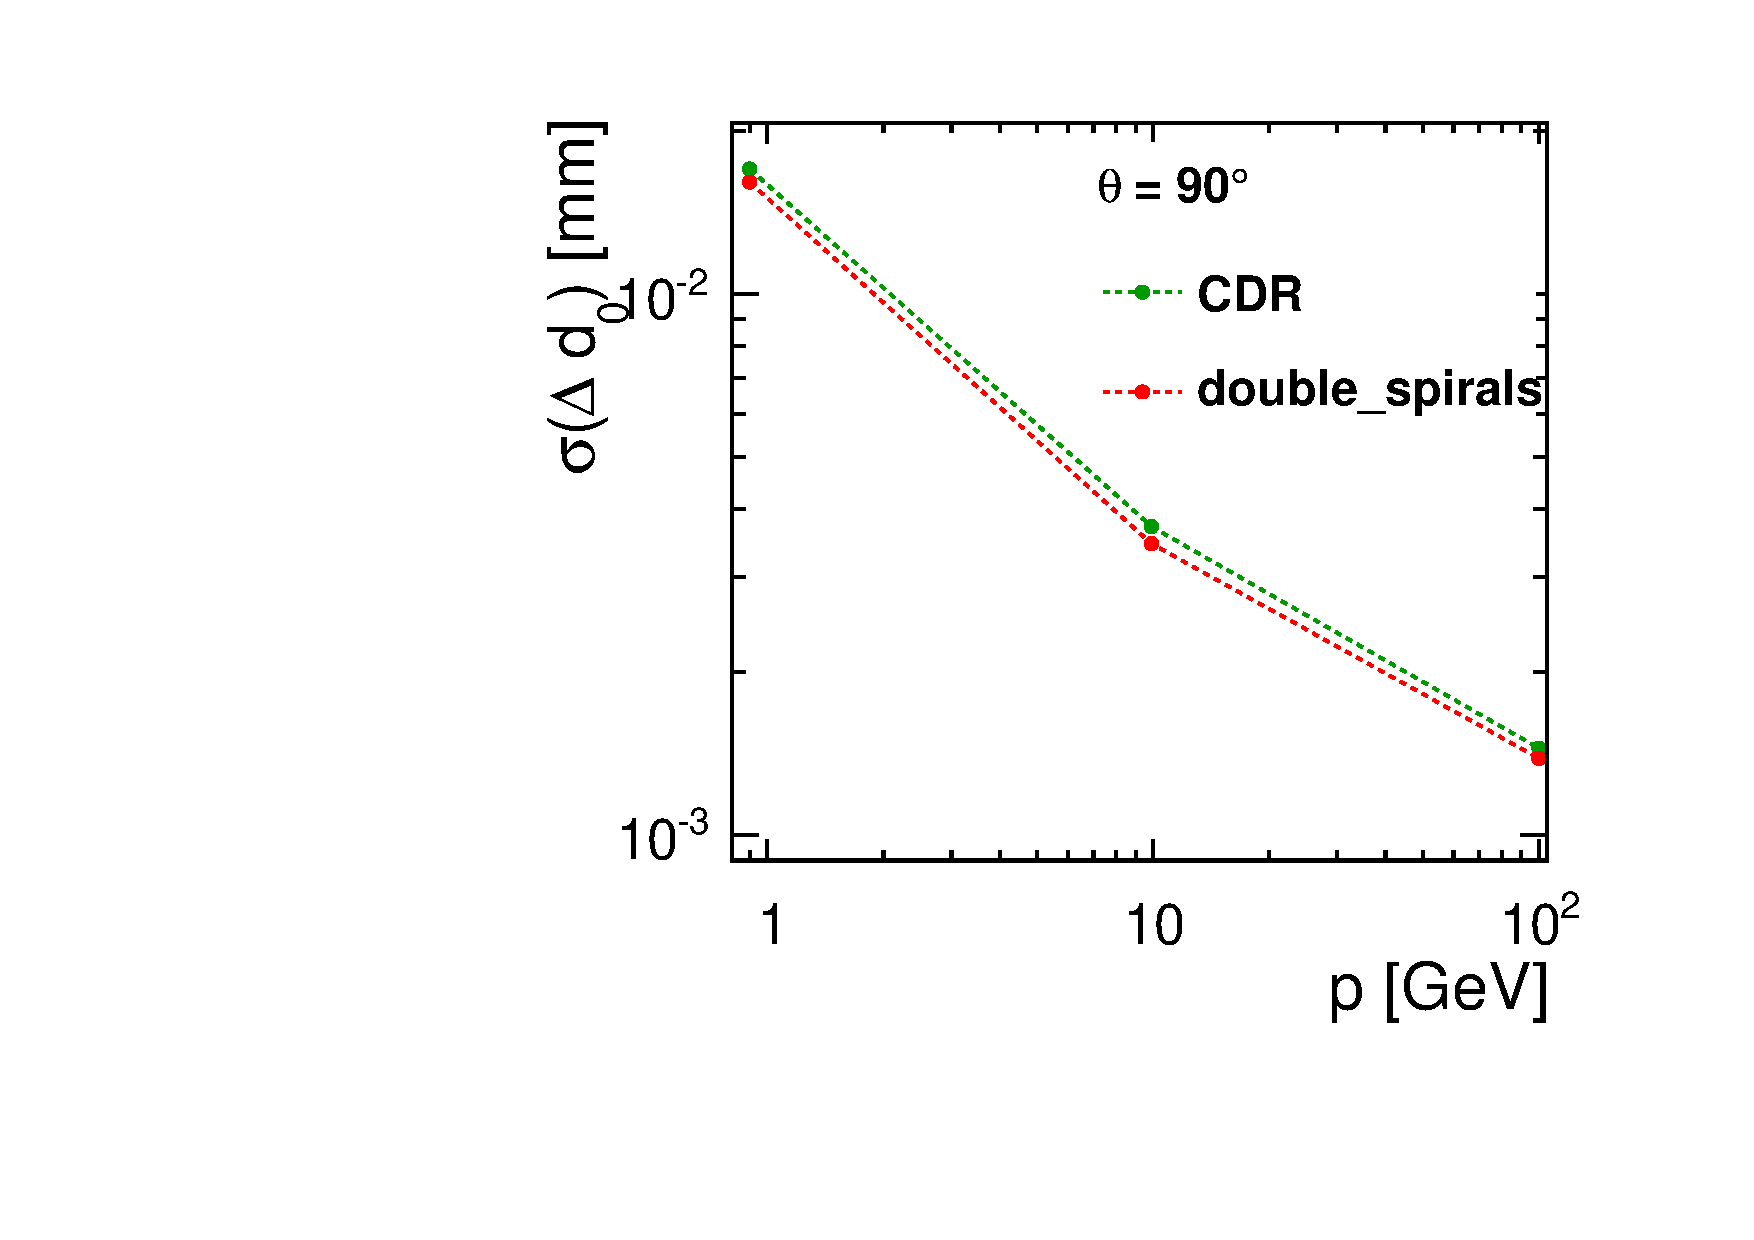
\includegraphics[width=\textwidth]{Figures/Geometries/d0_resolution_double.pdf}
          \caption{Transverse impact-parameter resolution}
          \label{}
        \end{subfigure}
        ~
        \begin{subfigure}[b]{\textwidth}
          \centering
          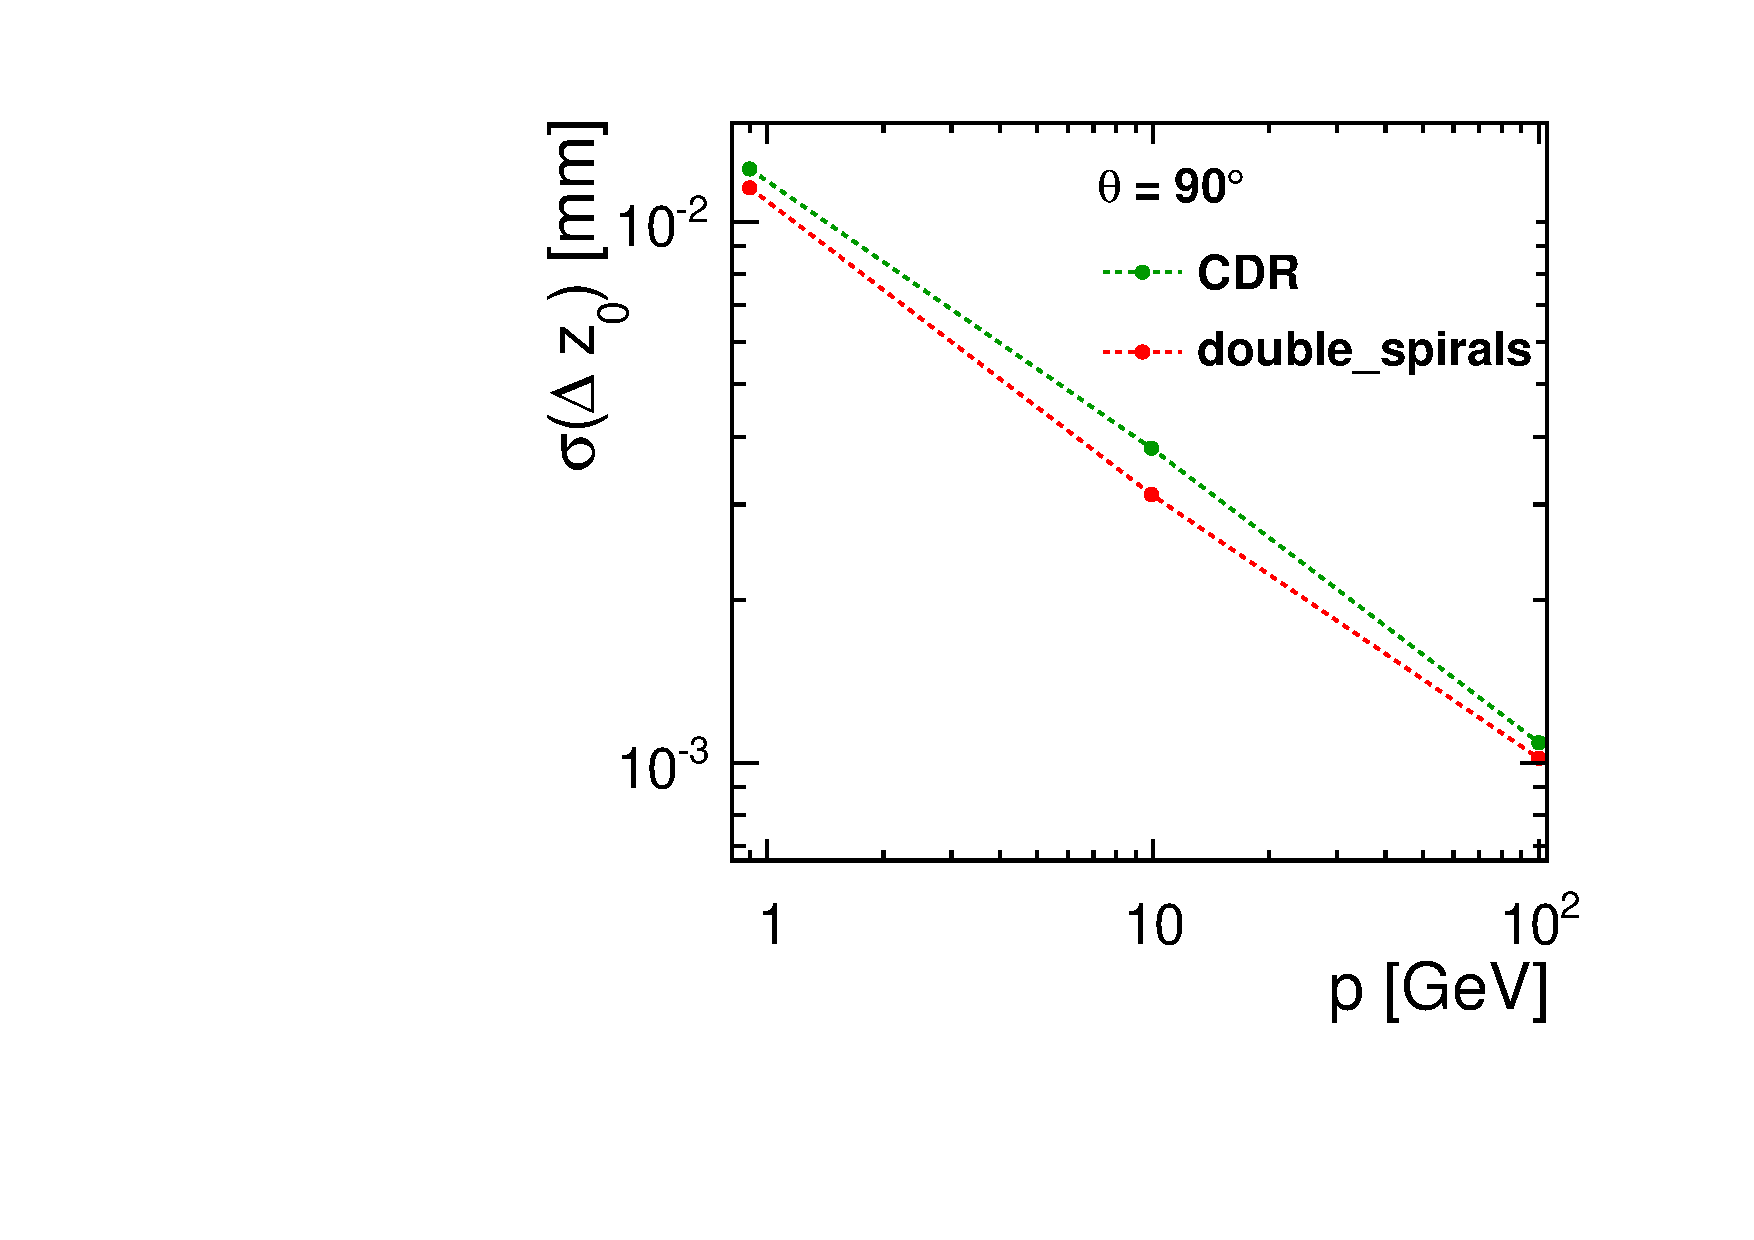
\includegraphics[width=0.4\textwidth]{Figures/Geometries/z0_resolution_double.pdf}
          \caption{Longitudinal impact-parameter resolution}
          \label{}
        \end{subfigure}
        \caption{(a) Momentum, (b) transverse impact-parameter and
          (c) longitudinal impact-parameter resolutions for the CDR and
          the {\it double\_spirals} geometries for singles muons at $\theta = 90^\circ$.}\label{fig:doubleLayerRes}
\end{figure}

We can conclude that the use of double-layered modules with 6 sensors in the barrel slightly improves the $d_0$ and $z_0$ resolutions, compared to the geometry with 5 single layers (CDR and \textit{spirals} geometries).

\newpage

\subsection{The \emph{double\_spirals\_v2} geometry}
The impact of the \begin{it}double\_spirals\_v2\end{it} geometry on the tracking performance is studied in the barrel and the endcap regions using single muons with polar angles of $\theta=90^{\circ}$ and $\theta=20^{\circ}$ in Figures~\ref{fig:doubleSpiralsV2Res90} and \ref{fig:doubleSpiralsV2Res20}, respectively. For muons at $\theta=20^{\circ}$, two different azimuthal angles $\phi=180^{\circ}$ and $\phi=225^{\circ}$ are considered which correspond to the first and the last module of the first endcap layer.
The impact of the material budget on the transverse and longitudinal impact-parameter resolutions is more visible in the barrel region.

\begin{figure}[H]
        \centering
        \begin{subfigure}[b]{0.5\textwidth}
          \centering
          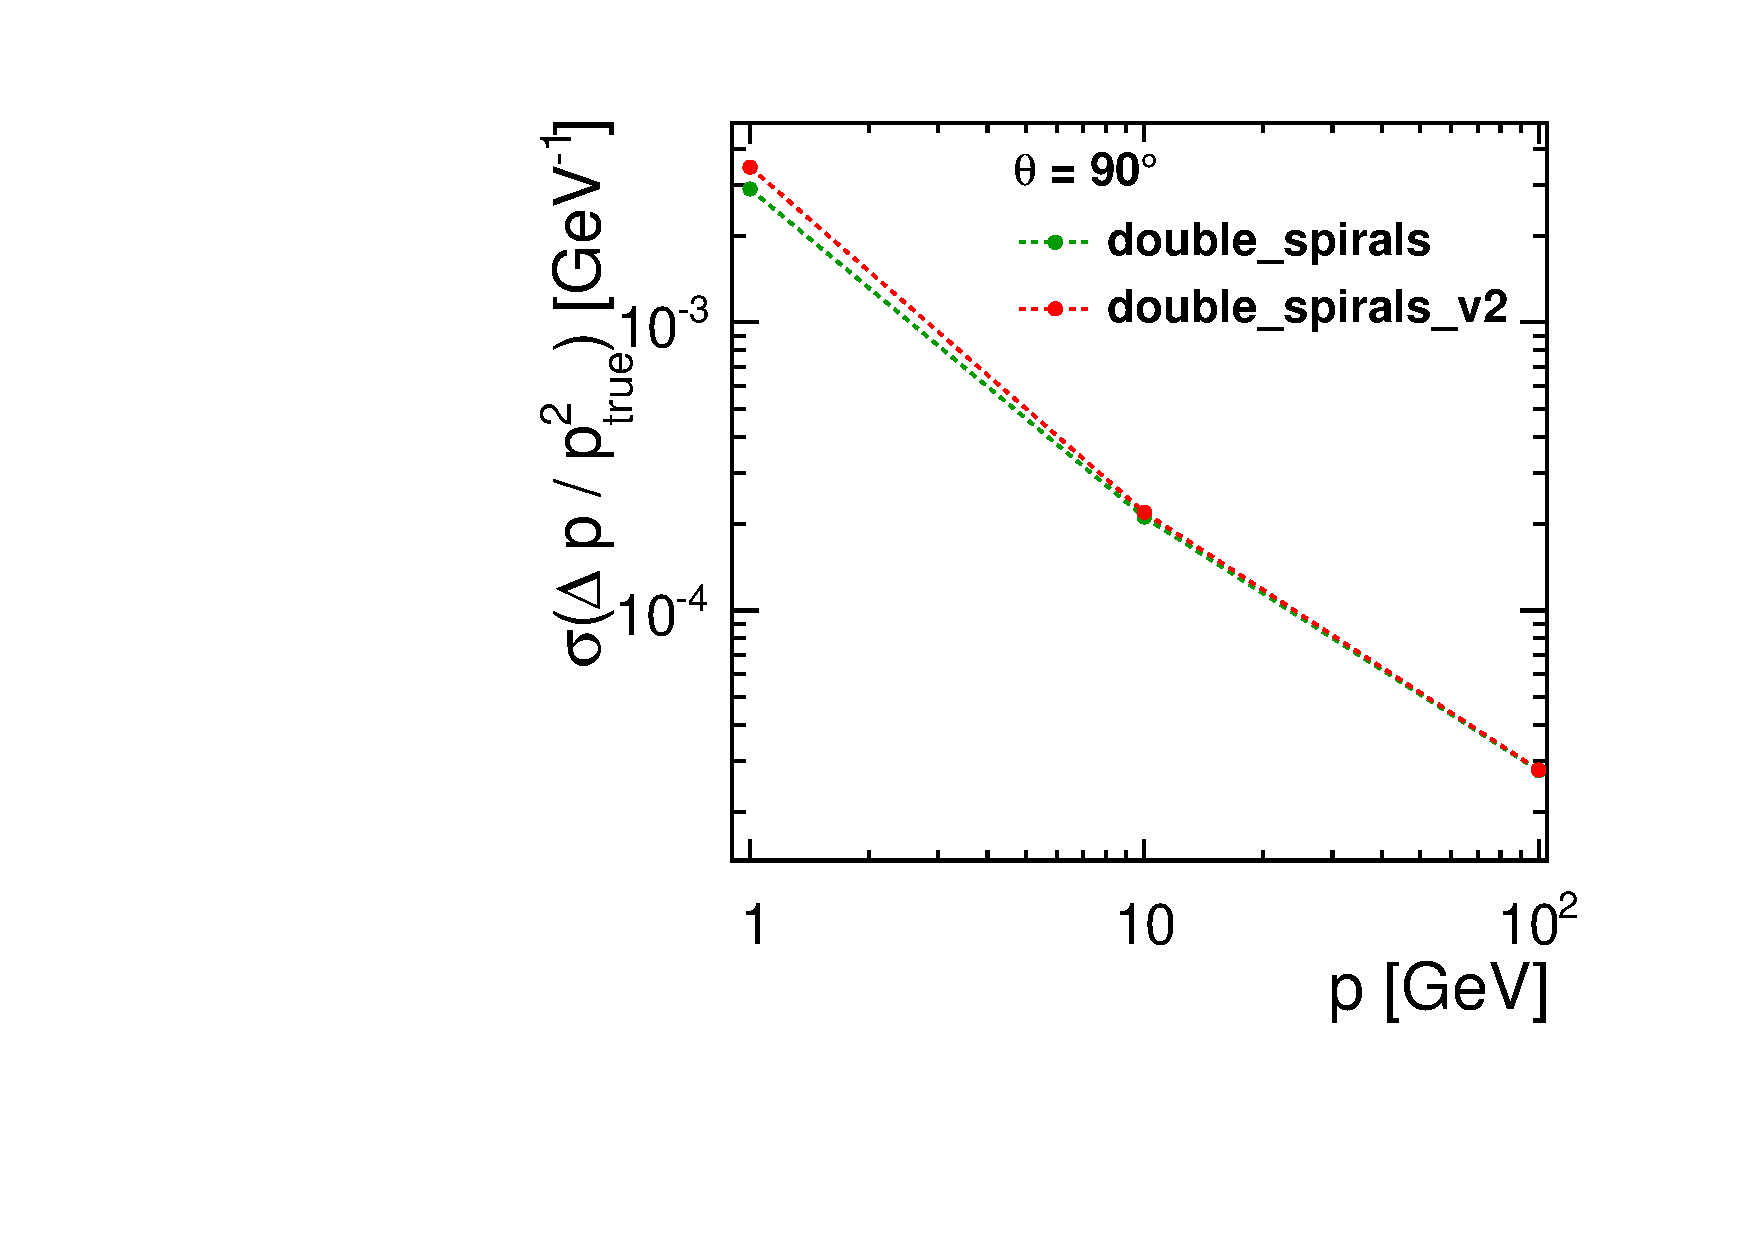
\includegraphics[width=\textwidth]{Figures/Geometries/p_resolution_double_spirals_v2_theta90.pdf}
          \caption{Momentum resolution}
          \label{}
        \end{subfigure}%
        ~ 
        \begin{subfigure}[b]{0.5\textwidth}
          \centering
          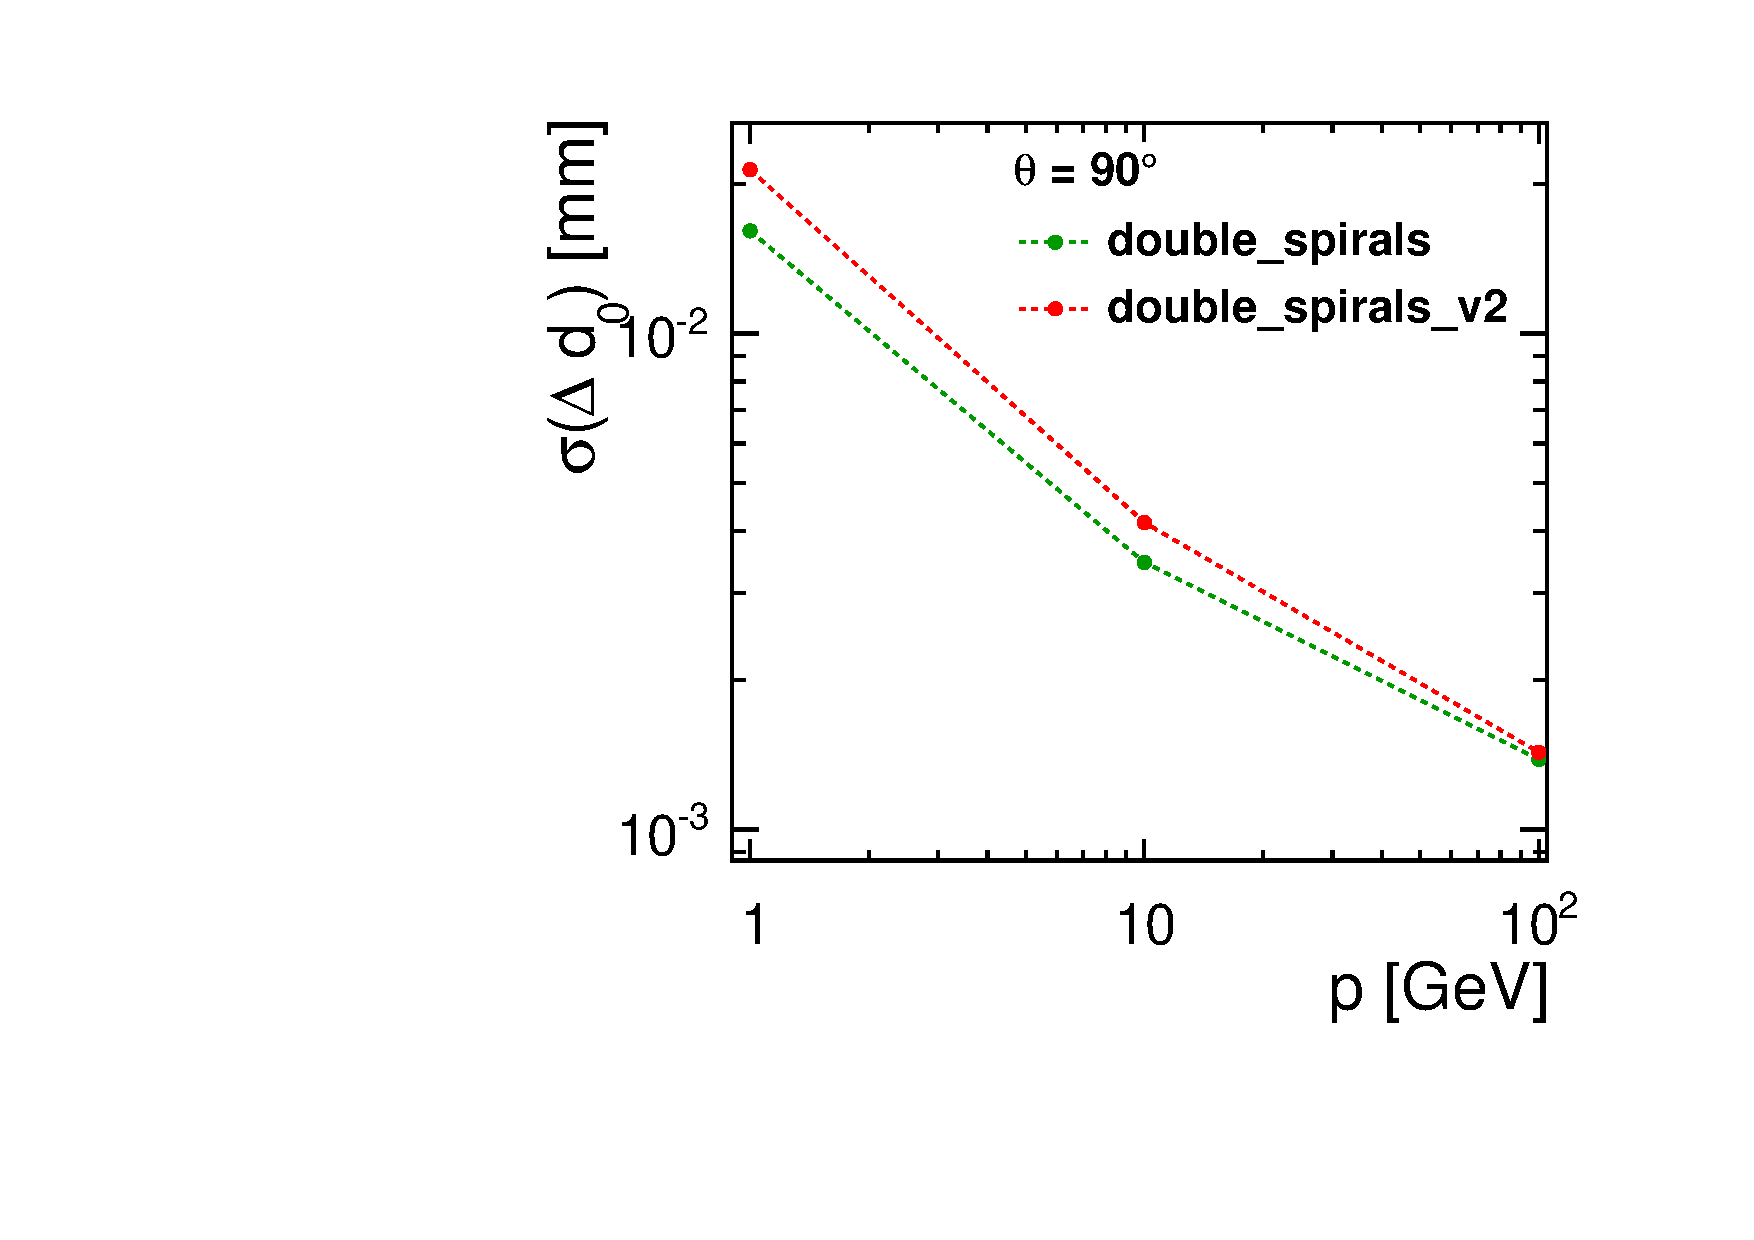
\includegraphics[width=\textwidth]{Figures/Geometries/d0_resolution_double_spirals_v2_theta90.pdf}
          \caption{Transverse impact-parameter resolution}
          \label{}
        \end{subfigure}
        ~
        \begin{subfigure}[b]{\textwidth}
          \centering
          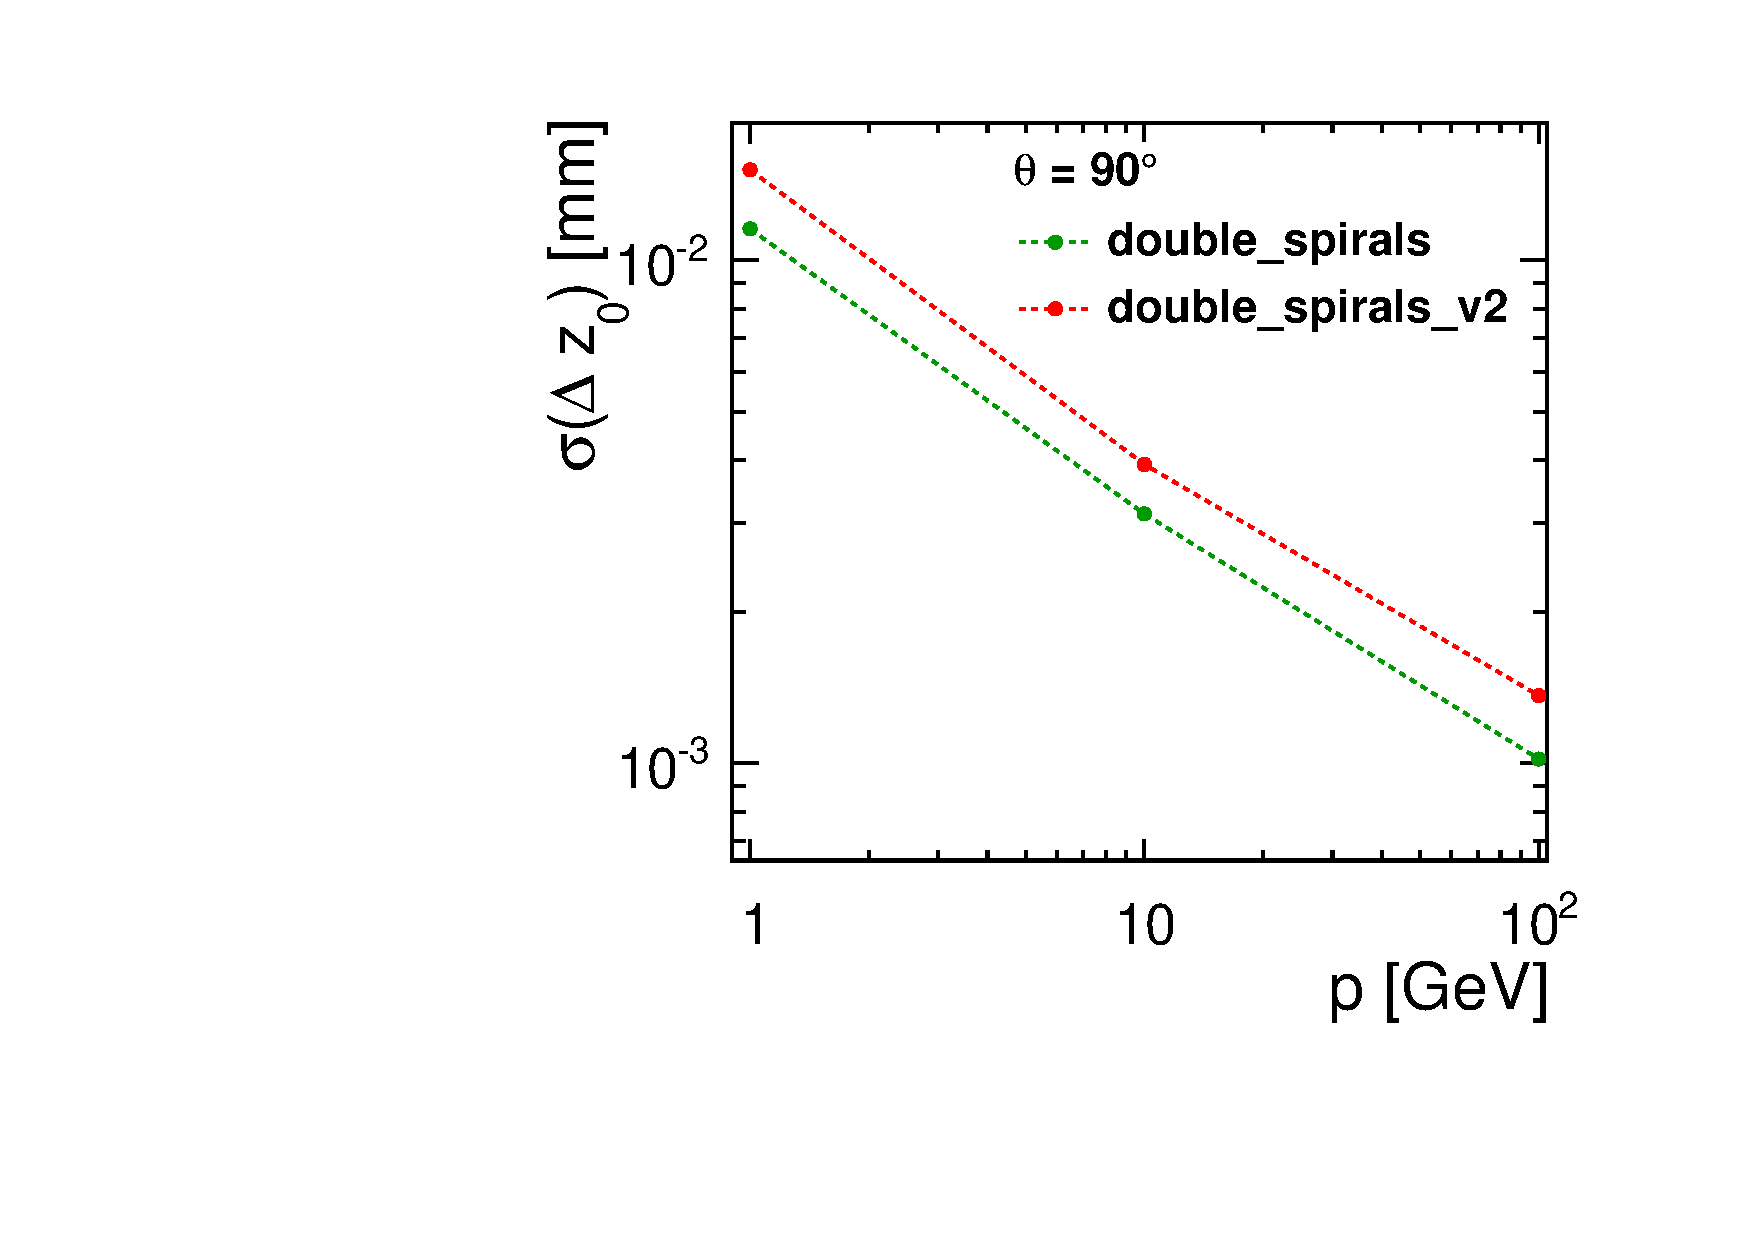
\includegraphics[width=0.5\textwidth]{Figures/Geometries/z0_resolution_double_spirals_v2_theta90.pdf}
          \caption{Longitudinal impact-parameter resolution}
          \label{}
        \end{subfigure}
        \caption{(a) Momentum, (b) transverse impact-parameter and
          (c) longitudinal impact-parameter resolutions for the {\it
            double\_spirals} and the {\it double\_spirals\_v2} geometries for singles muons at $\theta = 90^\circ$.}\label{fig:doubleSpiralsV2Res90}
\end{figure}

\begin{figure}[H]
        \centering
        \begin{subfigure}[b]{0.5\textwidth}
          \centering
          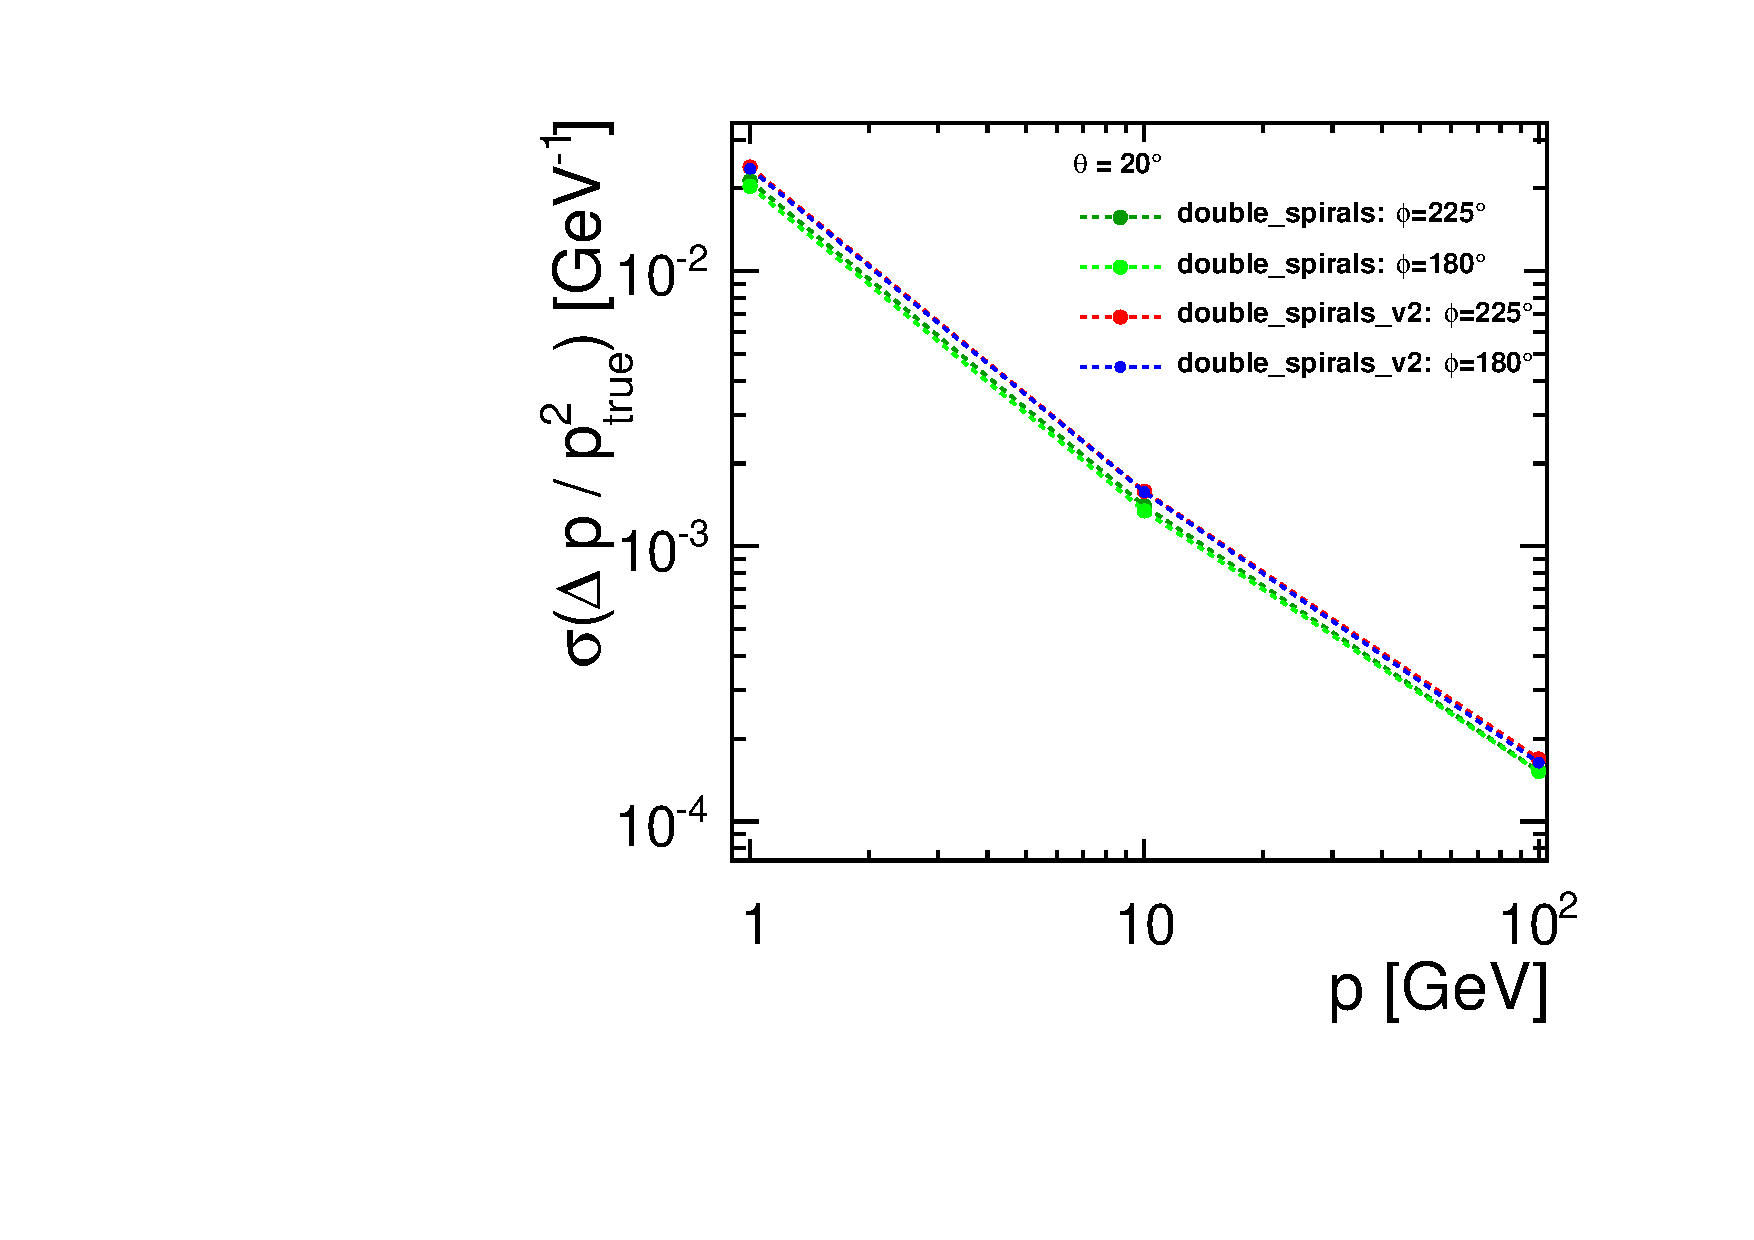
\includegraphics[width=\textwidth]{Figures/Geometries/p_resolution_double_spirals_v2_theta20.pdf}
          \caption{Momentum resolution}
          \label{}
        \end{subfigure}%
        ~ 
        \begin{subfigure}[b]{0.5\textwidth}
          \centering
          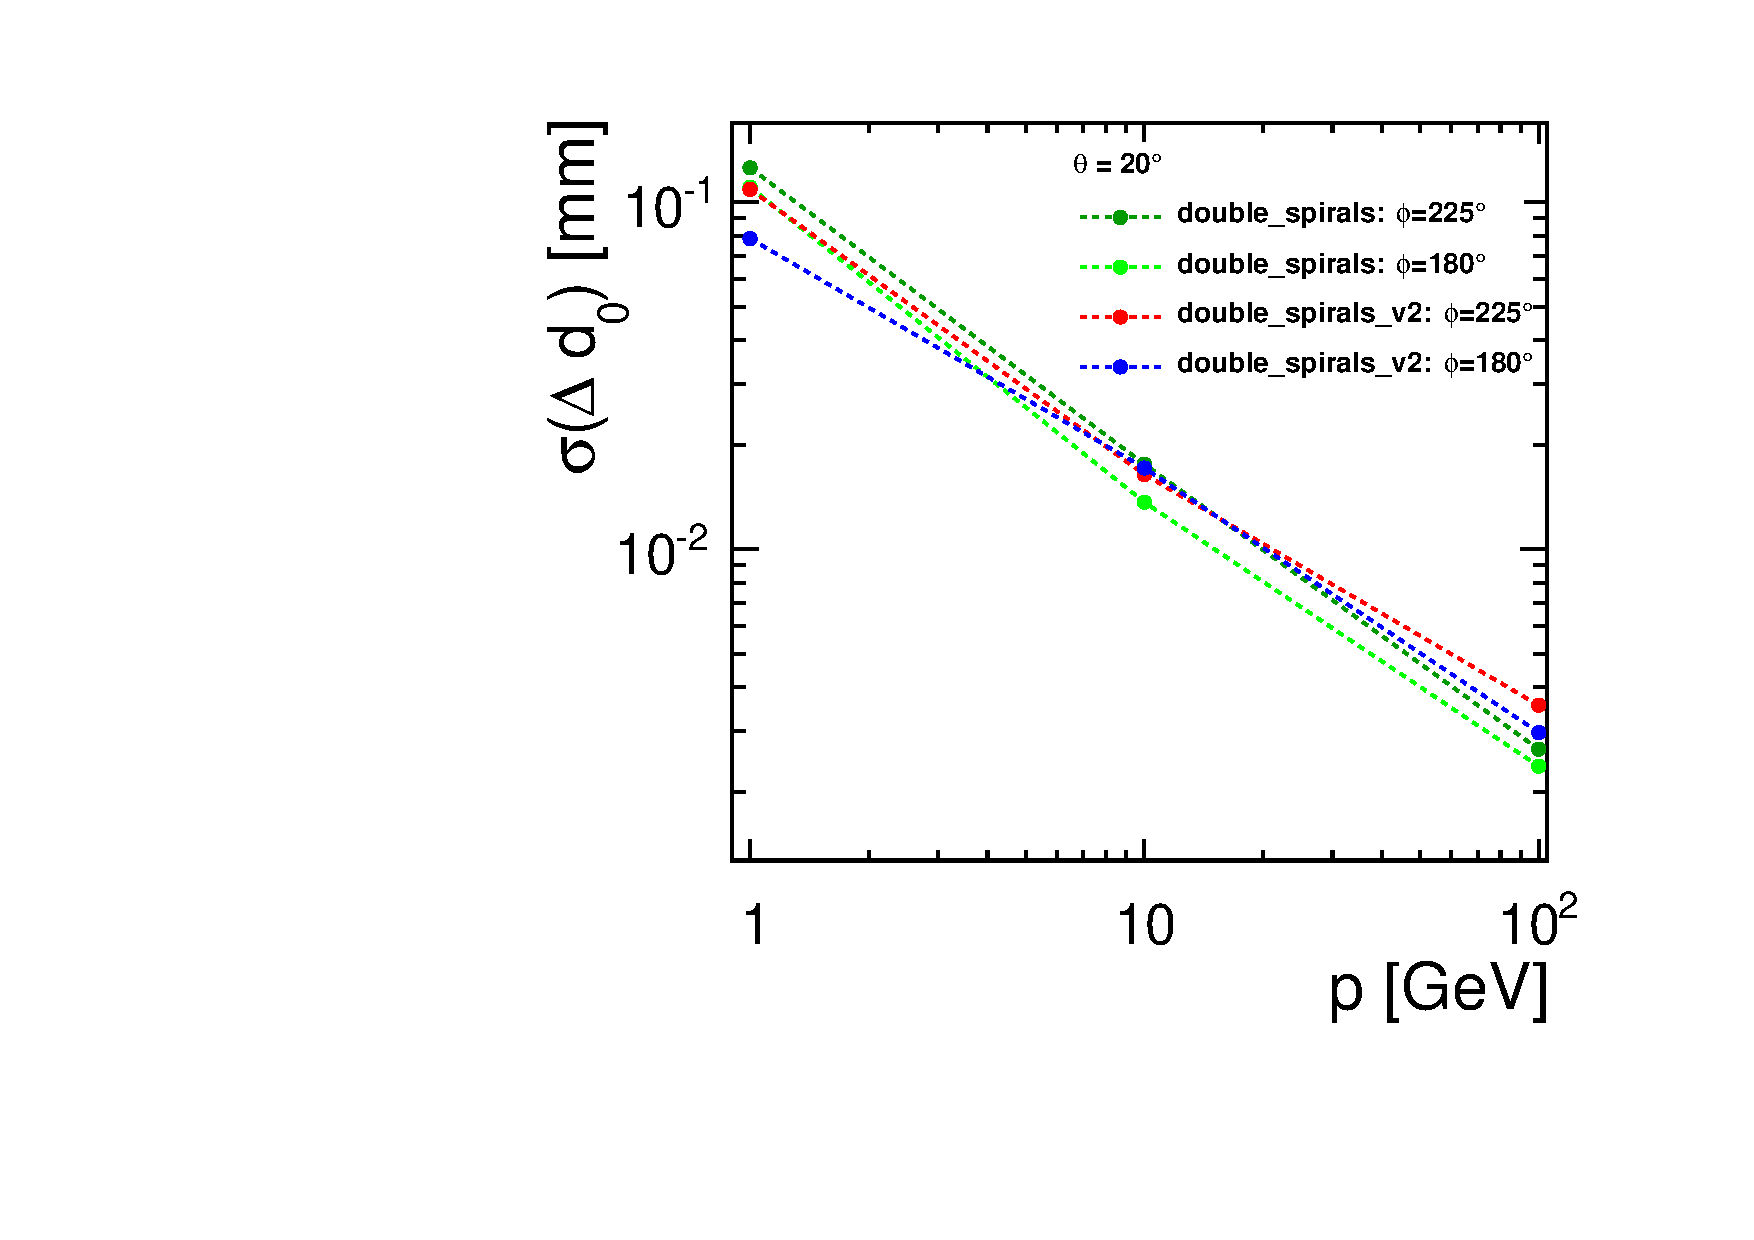
\includegraphics[width=\textwidth]{Figures/Geometries/d0_resolution_double_spirals_v2_theta20.pdf}
          \caption{Transverse impact-parameter resolution}
          \label{}
        \end{subfigure}
        ~
        \begin{subfigure}[b]{\textwidth}
          \centering
          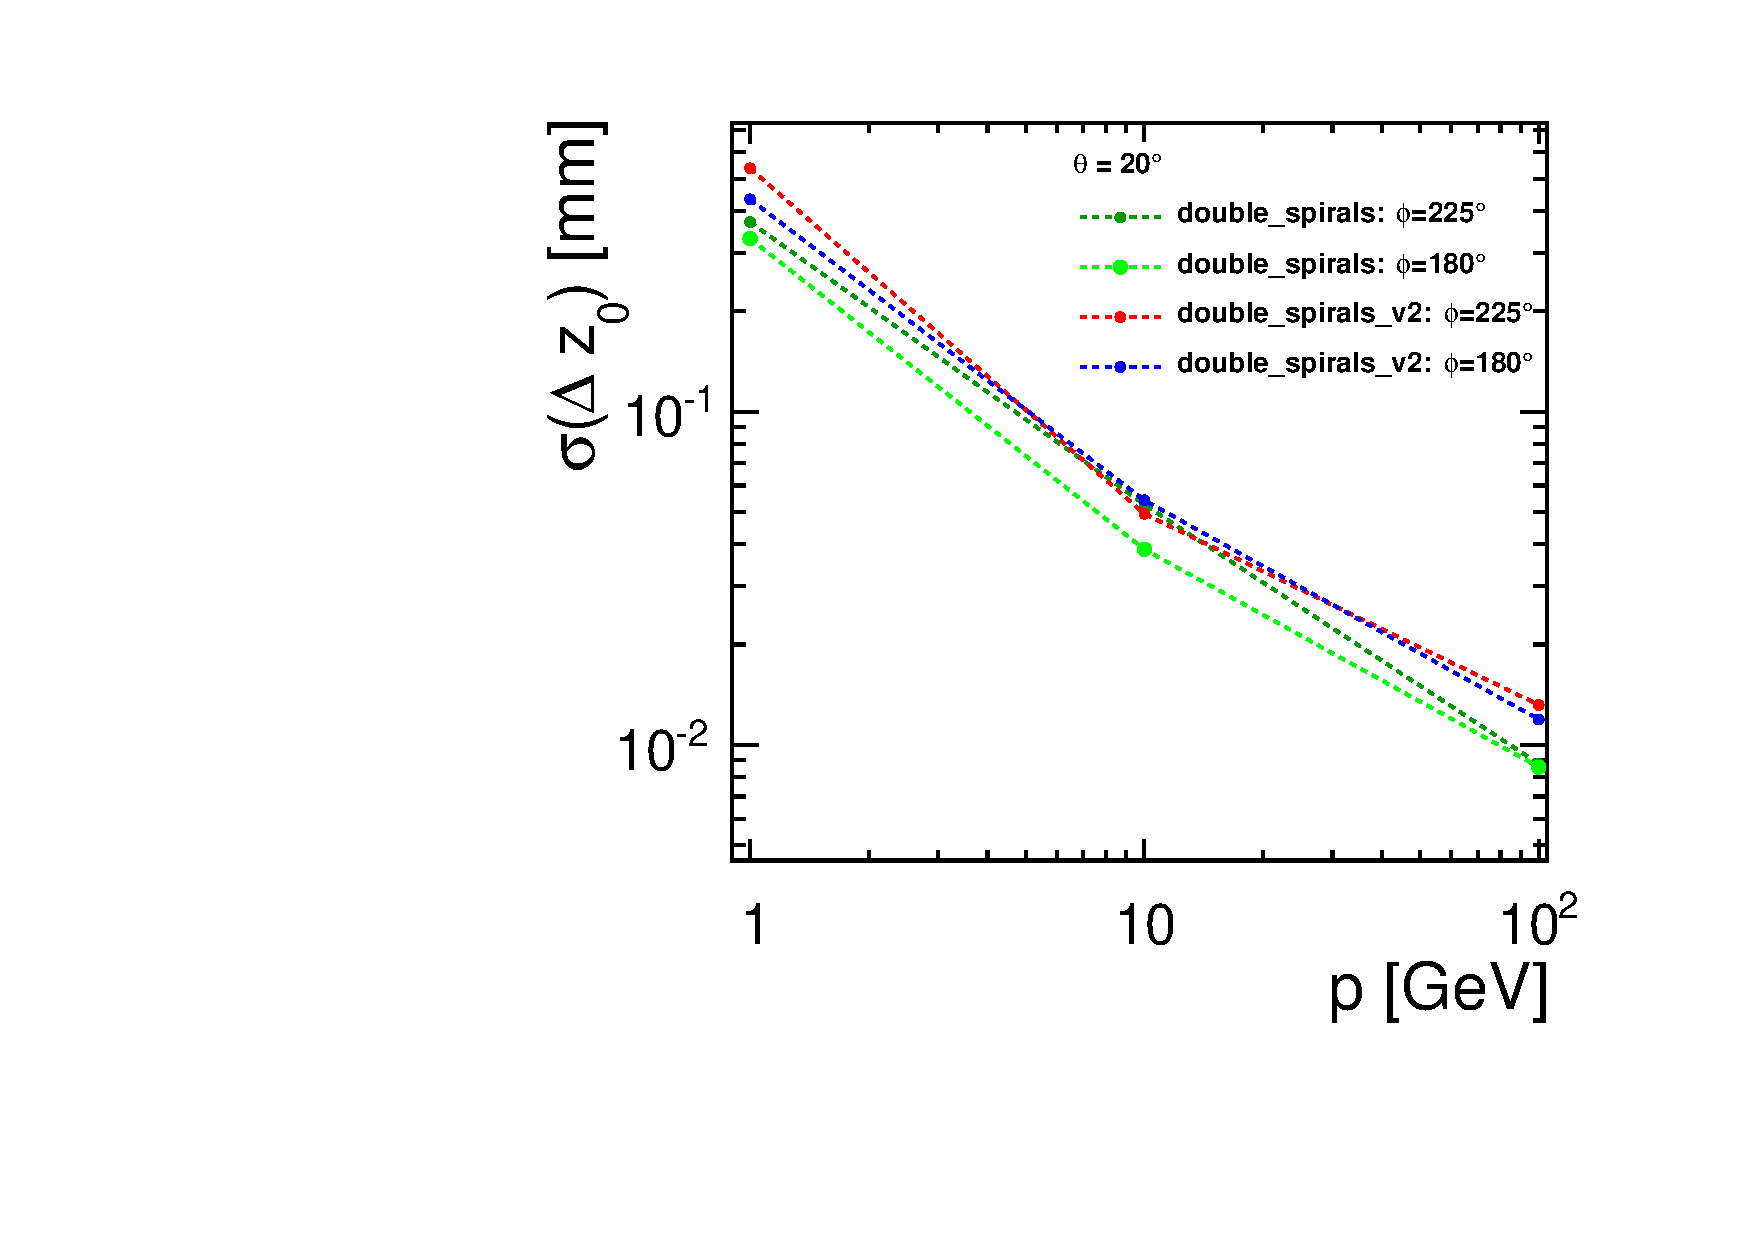
\includegraphics[width=0.5\textwidth]{Figures/Geometries/z0_resolution_double_spirals_v2_theta20.pdf}
          \caption{Longitudinal impact-parameter resolution}
          \label{}
        \end{subfigure}
        \caption{(a) Momentum, (b) transverse impact-parameter and
          (c) longitudinal impact-parameter resolutions for the
          {\it double\_spirals} and the {\it double\_spirals\_v2} geometries for
          singles muons at $\theta = 20^\circ$ with azimuthal angles
          of  $\phi = 225^\circ$ or $\phi = 180^\circ$.}\label{fig:doubleSpiralsV2Res20}
\end{figure}
